\documentclass{article}
\usepackage{tikz}
\usetikzlibrary{arrows}

\begin{document}

\begin{figure}
\centering
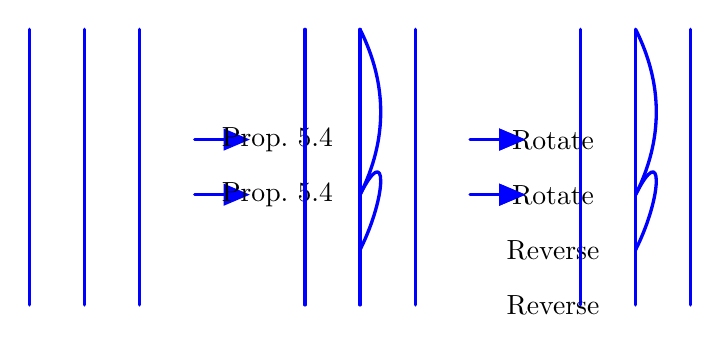
\begin{tikzpicture}[line cap=round, line join=round, >=triangle 45, x=0.7cm, y=0.7cm]

% First row of diagrams
\draw[blue, very thick] (0,0) -- (0,4);
\draw[blue, very thick] (1,0) -- (1,4);
\draw[blue, very thick] (2,0) -- (2,4);
\draw[->, blue, very thick] (3,2) -- (4,2);
\node at (4.5,2) {Prop.\ 5.4};
\draw[blue, very thick] (5,0) -- (5,4);
\draw[blue, very thick] (6,0) -- (6,4);
\draw[blue, very thick] (7,0) -- (7,4);
\draw[blue, very thick] (6,1) .. controls (6.5,2) and (6.5,3) .. (6,4);
\draw[->, blue, very thick] (8,2) -- (9,2);
\node at (9.5,2) {Rotate};
\draw[blue, very thick] (10,0) -- (10,4);
\draw[blue, very thick] (11,0) -- (11,4);
\draw[blue, very thick] (12,0) -- (12,4);
\draw[blue, very thick] (11,1) .. controls (11.5,2) and (11.5,3) .. (11,4);
\draw[<- , blue, very thick] (9,2) -- (8,2);
\node at (9.5,0) {Reverse};

% Second row of diagrams
\draw[blue, very thick] (0,-1) -- (0,3);
\draw[blue, very thick] (1,-1) -- (1,3);
\draw[blue, very thick] (2,-1) -- (2,3);
\draw[->, blue, very thick] (3,1) -- (4,1);
\node at (4.5,1) {Prop.\ 5.4};
\draw[blue, very thick] (5,-1) -- (5,3);
\draw[blue, very thick] (6,-1) -- (6,3);
\draw[blue, very thick] (7,-1) -- (7,3);
\draw[blue, very thick] (6,-0) .. controls (6.5,1) and (6.5,2) .. (6,1);
\draw[->, blue, very thick] (8,1) -- (9,1);
\node at (9.5,1) {Rotate};
\draw[blue, very thick] (10,-1) -- (10,3);
\draw[blue, very thick] (11,-1) -- (11,3);
\draw[blue, very thick] (12,-1) -- (12,3);
\draw[blue, very thick] (11,0) .. controls (11.5,1) and (11.5,2) .. (11,1);
\draw[<- , blue, very thick] (9,1) -- (8,1);
\node at (9.5,-1) {Reverse};

\end{tikzpicture}
\end{figure}

\end{document}